\documentclass[11pt]{article}
%Gummi|065|=)
\title{\textbf{Welcome to Gummi 0.6.6}}
\author{Alexander van der Meij\\
		Wei-Ning Huang\\
		Dion Timmermann}
\date{}
\usepackage{graphicx}
\usepackage{amsmath}
\usepackage{braket}

\begin{document}

\maketitle
\subsubsection{The  classical lossless beam splitter}
This section is inspired in the beam splitter description presented in \cite{Loudon} and \cite{leonhartd}\footnote{We are assuming monochromatic light that is only one mode}, in this thesis we will consider ideal beam splitters which are reversible and lossless devices, this device has two inputs and two outputs, so two input beams may interfere to produce two outgoing beams. A beam splitter is usually a dielectric interface that is birefringent inside a cube as the Fig.1 shows: 

\begin{figure}[h!]
\centering
\includegraphics[width=5 cm,height=5 cm]{images/bS.png}
\caption{A Beam splitter cube}
\label{fig:BS2}
\end{figure}

When we talk about a laser beam in classical electrodynamics we express it as an electric field, When going through a linear medium the outgoing fields can be written as a linear combination of the input fields satisfying boundary conditions \cite{jackson}. As we are dealing with 2 inputs and two outputs this can be written as:

\begin{equation}
\begin{pmatrix} E_{1}' \\ E_{2}' \end{pmatrix}=B\begin{pmatrix} E_{1} \\ E_{2} \end{pmatrix}.
\end{equation}

The linear transformation $B$ is described by a matrix:

\begin{equation}
B=\begin{pmatrix} B_{11}& B_{12} \\B_{21} & B_{22}. \end{pmatrix}
\end{equation}

Conditions on the coefficients on this matrix can be found by asking for the total intensity to be conserved (since it's lossless it should be full-filed), that is:

\begin{align}
&I_{1}'+I_{2}'=I_{1}+I_{2}, \\
&I_{1}'\propto|B_{11} E_{1}|^{2}+|B_{12} E_{2}|^{2}+B_{11} B_{12}* E_{1} E_{2}*+B_{11}* B_{12} E_{1}* E_{2}, \\
&I_{2}'\propto|B_{21} E_{1}|^{2}+|B_{22} E_{2}|^{2}+B_{21} B_{22}* E_{1} E_{2}*+B_{21}* B_{22} E_{1}* E_{2},\\
&|E_{1}|^{2}+|E_{2}|^{2}=(|B_{21}|^{2}+|B_{11}|^{2})|E_{1}|^{2}+(|B_{12}|^{2}+|B_{22}|^{2})|E_{2}|^{2}+\\
&(B_{21} B_{22}*+B_{11} B_{12}*)E_{1} E_{2}*+(B_{21}* B_{22}+B_{11}* B_{12})E_{1}* E_{2}.
\end{align}

So from conservation of intensity (energy) we obtain the following relationships:

\begin{align}
&|B_{12}|^{2}+|B_{22}|^{2}=|B_{21}|^{2}+|B_{11}|^{2}=1,\\
&B_{21}* B_{22}+B_{11}* B_{12}=0.
\end{align}

From these relations it follows that the matrix is unitary \footnote{From these set of equations one can derive yet another constraint on the coefficients $B_{21}* B_{11}+B_{22}* B_{12}=0$ can be obtained this is because $B^{\dagger}B=B^{\dagger}B=\mathbb{1}$}, We will write this matrix in terms of the reflectivity $\rho$ and the transmissivity $\tau$ that follow the relationship:

\begin{equation}
|\tau|^{2}+|\rho|^{2}=1.
\end{equation}
  
 In the classical case the transformation is usually written as:
 
 \begin{equation}
 B=\begin{pmatrix} \tau & \rho \\ -\rho & \tau \end{pmatrix}.
 \end{equation} 


so that 

\begin{equation}
\begin{pmatrix} E_{1}' \\ E_{2}' \end{pmatrix}=\begin{pmatrix} \tau & \rho \\ -\rho & \tau \end{pmatrix} \begin{pmatrix} E_{1} \\ E_{2} \end{pmatrix}.
\end{equation}




\subsubsection{The quantum lossless beam splitter}

We will now develop the quantum theory of a lossless beam splitter. To do this we will first quantize the electric field and then build the theory\footnote{It should not be a surprise that we obtain basically the same theory as in the case of the classical beam splitter because it is quite typical that classical laws rule interference phenomena, going quantum often only affects the visibility, but does not modify the theory \cite{Leonhardt_2003} } 


The quantized electric field can be written as:

\begin{equation}
\mathbf{E}=i \hat{\epsilon}N w \left( \alpha e^{i (\mathbf{k \cdot r}-w t)}+\alpha^{*} e^{-i (\mathbf{k \cdot r}-w t)} \right)
\end{equation}

Where $\alpha$ is known as the complex wave amplitude, to make our theoretical model of a beam splitter as general as possible, let us describe the device as a four-port device, a black box with two input and two output ports having certain properties.

If two coherent light beams with complex wave amplitudes $\alpha_{1}$ and $\alpha_{2}$ enter the beam splitter we simply expect the output complex wave amplitude  are superimposed according to a linear transformation that we will call $B$ so that:

\begin{equation}
\begin{pmatrix} \alpha_{1}' \\ \alpha_{2}' \end{pmatrix}=B\begin{pmatrix} \alpha_{1} \\ \alpha_{2} \end{pmatrix}
\end{equation}

When we quantize the electric field the complex wave amplitude $\alpha$ is promoted to a ladder operator. Once quantized this becomes:

\begin{equation}
\begin{pmatrix} \hat{a}_{1}' \\ \hat{a}_{2}' \end{pmatrix}=B\begin{pmatrix} \hat{a}_{1} \\ \hat{a}_{2} \end{pmatrix}
\label{eq:amplitudes}
\end{equation}

As this equation describes the change of the ladder operators in the process, it corresponds to the Heisenberg picture. Assuming the incoming and outgoing beams are both independent bosonic modes, we can obtain some properties of the $B$ matrix because the ladder operators must obey:

\begin{align}
&[\hat{a}'_{\nu},\hat{a}'_{\mu}]=[\hat{a}_{\nu},\hat{a}_{\mu}]=0,\\
&[\hat{a}'_{\nu},\hat{a}'^{\dagger}_{\mu}]=[\hat{a}_{\nu},\hat{a}^{\dagger}_{\mu}]=\delta_{\mu \nu}.
\label{commutators}
\end{align}

From Eq.\ref{eq:amplitudes} it follows that:

\begin{align}
&\hat{a}'_{\mu}=B_{\mu 1}\hat{a}_{1}+B_{\mu 2} \hat{a}_{2}, \\
&\hat{a}'^{\dagger}_{\mu}=B_{\mu 1}^{*}\hat{a}^{\dagger}_{1}+B_{\mu 2}^{*} \hat{a}^{\dagger}_{2}. 
\label{combined amplitudes}
\end{align}

Then we use the commutation relations to find constraints on the elements of the $B$ matrix, using Eq. \ref{combined amplitudes} and Eq. \ref{commutators} we find that:

\begin{equation}
   [\hat{a}'_{\nu},\hat{a}'^{\dagger}_{\mu}]=B_{\nu 1} B_{\mu 1}^{*}+B_{\nu 2} B_{\mu 2}^{*} .
\end{equation}

Substituting for all possible values of $\nu$ and $\mu$ we find the following relationships:

\begin{equation}
|B_{11}|^{2}+|B_{12}|^{2}=|B_{21}|^{2}+|B_{22}|^{2}=1 ,\qquad B_{11} B_{21}^{*}+B_{12} B_{22}^{*}=0
\end{equation}

Which indicate that the B transformation is unitary, something we expected of a lossless device. The most general form of a unitary $2x2$ matrix is\cite{leonhardt}:


\begin{equation}
B=e^{\Lambda} \begin{pmatrix} e^{i\frac{\phi}{2}} & 0 \\ 0 & e^{-i\frac{\phi}{2}} \end{pmatrix} \begin{pmatrix} \cos(\theta) &  \sin(\theta) \\ - \sin(\theta) & \cos(\theta) \end{pmatrix} \begin{pmatrix} e^{i\frac{\psi}{2}} & 0 \\ 0 & e^{-i\frac{\psi}{2}} \end{pmatrix} \label{unitary}
\end{equation}

Note that our analysis so far is valid for any lossless 4-port linear device, furthermore from \ref{unitary} we can see that any 4-port device can be considered as acting in three steps \footnote{A phase shifter is denoted by $P_{\phi}=e^{i \frac{\phi}{2}}\begin{pmatrix}e^{i \frac{\phi}{2}} & 0 \\ e^{-i \frac{\phi}{2}} &0 \end{pmatrix}$}. First the phases of the incident modes are changed, then the amplitudes are mixed(rotated) and then the phases change again. In most cases we can adjust the reference phases such that only the rotation is important, so this is the key feature of 4-ports, that is why from now on we will parametrize our beam splitter($BS$) as\footnote{This corresponds to $\Lambda=0$,$\phi=-\psi=\frac{\pi}{2}$}:


\begin{equation} 
BS=\begin{pmatrix} \cos(\theta) & i \sin(\theta) \\ i \sin(\theta) & \cos(\theta) \end{pmatrix}
\end{equation}



In the quantum case we are just interested in the single photon state so let us now analyze this optical element in the fock basis. In the heisenberg picture operators evolve via the evolution operator:

\begin{equation}
\begin{pmatrix} \hat{a}'_{1} \\ \hat{a}'_{2}\end{pmatrix}=\hat{U}^{\dagger}_{B} \begin{pmatrix} \hat{a}_{1} \\ \hat{a}_{2}\end{pmatrix} \hat{U}_{B} 
\label{Heisenberg}
\end{equation}

A Fock state $\ket{n_{1},n_{2}}$ can be generated from a vacuum state\footnote{When one of the inputs does not have a beam what enters the beam splitter is a vacuum state $\ket{0,0}$} by:

\begin{equation}
    \ket{n_{1},n_{2}}=\frac{1}{\sqrt{n_{1}! n_{2}!}} \hat{a}^{\dagger}^{n_{2}}_{1}\hat{a}^{\dagger}^{n_{2}}_{2} \ket{0,0}
\end{equation}

In the Schrodinger picture a vacuum state evolves by:

\begin{equation}
    \ket{\psi}'=U_{B}\ket{\psi} \qquad
    \ket{0,0}'=U_{B}\ket{0,0}
    \label{evolution}
\end{equation}

So now let us see the evolution of a $\ket{n_{1},n_{2}}'$\footnote{ Vacuum states are equivalent they are vacuum, we apply the transformed operators on the vacuum because we are looking for the output}:

\begin{equation}
\ket{n_{1},n_{2}}'=\frac{U_{B}}{\sqrt{n_{1}! n_{2}!}} \hat{a}'^{\dagger}^{n_{2}}_{1}\hat{a}'^{\dagger}^{n_{2}}_{2} \ket{0,0}'
\end{equation}

From Eq. \ref{Heisenberg}, Eq. \ref{eq:amplitudes} and Eq. \ref{evolution} we can obtain:

\begin{equation}
\ket{n_{1},n_{2}}' &&=\frac{U_{B}}{\sqrt{n_{1}! n_{2}!}} \hat{a}'^{\dagger}^{n_{2}}_{1}\hat{a}'^{\dagger}^{n_{2}}_{2} U^{\dagger}_{B}\ket{0,0}'
\end{equation}
\begin{equation}
\ket{n_{1},n_{2}} && =\frac{1}{\sqrt{n_{1}! n_{2}!}} \hat{a}^{\dagger}^{n_{2}}_{1}\hat{a}^{\dagger}^{n_{2}}_{2}\ket{0,0}
\end{equation}

By writing the original ladder operators in terms of the transformed ladder operators, and applying Newton's binomial formula\footnote{We can do this because the operators commute in general this cannot be done} we arrive at the ``compact'' expression \footnote{ The binonial coefficient is $ \begin{pmatrix} n \\ k \end{pmatrix} =\frac{n!}{\sqrt{k!(n-k)!}}$}:

\begin{align*}
    \ket{n_{1},n_{2}}'=\frac{1}{\sqrt{n_{1}! n_{2}!}}\sum^{n_{1},n_{2}}_{k_{1},k_{2}=0}\begin{pmatrix} n_{1} \\ k_{1} \end{pmatrix}\begin{pmatrix} n_{2} \\ k_{2} \end{pmatrix} B_{11}^{n_{1}-k_{1}} B_{21}^{k_{1}} B_{12}^{n_{2}-k_{2}} B_{22}^{k_{2}} \\ \sqrt{(n_{1}+n_{2}-k_{1}-k_{2})!(k_{1}+k_{2})!} \ket{n_{1}+n_{2}-k_{1}-k_{2},k_{1}+k_{2}}
\end{align*}

Now let us consider one of the inputs is vacuum that is $n_{2}=0$ and $n_{1}=n$  and vice-versa:
\begin{align}
    \ket{n,0}'=\sum^{n}_{k=0} \sqrt{\frac{n!}{(n-k)!k!}} B_{11}^{n-k} B_{21}^{k} \ket{n-k,k}\\
        \ket{0,n}'=\sum^{n}_{k=0} \sqrt{\frac{n!}{(n-k)!k!}} B_{12}^{n-k} B_{22}^{k} \ket{n-k,k}
\end{align}

In this thesis we intend to work with single-photons, so that our case of interest is $n=1$,we run the sum to obtain:

\begin{align}
\ket{1,0}'=B_{11}\ket{1,0}+B_{21}\ket{0,1} \\
\ket{0,1}'=B_{12}\ket{1,0}+B_{22}\ket{0,1}
\label{basis}
\end{align}


From Eq. \ref{basis} we can see that the case of the single-photon can be written in terms of the BS matrix if we define an appropriate basis to describe the system. The one we will use is the Horizontal-Vertical computational basis.We will use:

 \begin{equation}
 \ket{1}=\ket{1}_{h}\ket{0}_{v}=\begin{pmatrix} 1 \\0\end{pmatrix}
 \end{equation} 

 meaning one photon in the horizontal path and vacuum in the vertical path
 
 \begin{equation}
 \ket{2}=\ket{0}_{h}\ket{1}_{v}=\begin{pmatrix} 0 \\1 \end{pmatrix}
 \end{equation}
 
meaning vacuum  in the horizontal path and one photon in the vertical path, so then Eq. \ref{basis} become:
\begin{equation}
\ket{out}=\begin{pmatrix} \cos(\theta) & i \sin(\theta) \\ i \sin(\theta) & \cos(\theta) \end{pmatrix} \ket{in},
\end{equation}

where $\ket{in}=\ket{1},\ket{2}$ and out is a linear combination of the vectors $\ket{1},\ket{2}$.A mirror in this basis(Horizontal-Vertical) simply flips the state and adds a phase: 
 
\begin{equation}
M=\begin{pmatrix} 0& e^{i\gamma}  \\ e^{i\gamma} & 0 \end{pmatrix}.
\end{equation}

We have now defined all the things we need in order to analyze the interferometer in the classical and quantum case, which we will do in the next sections

\end{document}
